\section{Messen von Kondensatoren}
Die Messung von Kapazit\"atswerten wird nach allen anderen Messungen als separater Teil mit einer Ladezeitmessung 
durchgef\"uhrt.
Die original Software vom Markus F. hat das mit einer Programm-Schleife gemacht, die den betreffenden digitalen
Eingangs Pin bis zu einer Signal\"anderung gelesen hat und dabei die Schleifendurchl\"aufe gez\"ahlt.
Dies hat den Nachteil, da"s die Aufl\"osung der Zeitmessung begrenzt ist durch die Gesamtzeit eines Schleifendurchlaufs.
Dies wurde \"ublicherweise in allen sechs Kombinationsm\"oglichkeiten f\"ur die drei Testpins durchgef\"uhrt.
Die aktuelle Software benutzt zwei verschiedene M\"oglichkeiten um die Ladezeit zu erhalten in nur drei
Kombinationsm\"oglichkeiten f\"ur die drei Testpins.
Die positive Seite ist nun immer die h\"ohere Testpin-Nummer.
Nur wenn die Kapazit\"at zusammen mit einer parallel geschalteten Diode gemessen wird,
kann die Polarit\"at die andere Richtung haben.

\subsection{Entladen der Kondensatoren}
Sie sollten die Kapazit\"aten immer entladen, bevor sie mit dem Tester verbunden werden.
Bevor irgendein Test gestartet wird, wird der Kondensator vom Tester immer noch einmal entladen.
Wenn die Spannung unter 1300mV ist, wird der Kondensator daf\"ur mit den angeschlossenen ADC Ports (Port C) kurzgeschlossen.
Ich glaube das ist legal, weil jeder Portausgang einen Innenwiderstand von ungef\"ahr \(20\Omega\) hat.
Die Abbildung 149 (Seite 258) im Atmega8 Datenblatt \cite{ATmega8} zeigt einen Spannungsabfall an Ausgabe-Pins von bis zu 2V.
Nat\"urlich kann ich nicht garantieren, da"s kein Schaden auftreten kann.
Ich habe die Funktion mit 15mF Kondensatoren sehr oft getestet und ich habe noch nie ein Problem bemerkt.
Der Strom sollte unter der spezifizierten Grenze von 40mA bleiben und reduziert sich schnell durch die Entladung.
Nat\"urlich kann ein Schaden entstehen, wenn Sie einen (Hochvolt-) Kondensator vor dem Anschlie"sen an den Tester nicht entladen.

\subsection{Messung von gro"sen Kapazit\"aten}
\label{sec:bigcap}
Eine Seite des Kondensators ist mit GND verbunden. Die andere Seite wird \"uber den \(680\Omega\) Widerstand f\"ur 10ms mit VCC verbunden.
Danach wird dieser Messpin auf Eingang geschaltet (Hochohmig).
Nach diesem Strompuls wird die Spannung am Kondensator stromlos gemessen.
Wenn die Spannung noch nicht den Minimalwert von 300mV erreicht hat, wird der 10 ms Ladepuls bis zu 499 Mal wiederholt.
Wenn nach 127 Pulsen (ungef\"ahr 2s) noch nicht eine Minimalspannung von 75mV erreicht ist, wird der Ladevorgang abgebrochen,
 weil die 300mV mit den verbleibenden Ladepulsen nie erreicht werden kann.
Abbildung~\ref{fig:bigcap} zeigt die drei Phasen der Kapazit\"atsbestimmung eines Kondensators.
Der Kapazit\"atswert wird dann berechnet aus der Ladepuls-Anzahl und der erreichten Ladespannung \"uber eine Tabelle.
Die Tabelle enth\"alt mit einem Spannungsabstand von 25mV die Faktoren, um aus der Ladezeit und der Spannung 
den Kapazit\"atswert zu bestimmen. 
Zwischenwerte der Spannung werden interpoliert.

\begin{figure}[H]
\centering

\includegraphics[]{../FIG/Bigcap.eps}
\caption{Kondensator Entladung und Ladung mit 10ms Ladepulsen bis Spannung \textgreater 300mV}
\label{fig:bigcap}
\end{figure}
Wegen der niedrigen Ladespannung wird die Messung viel schneller als bei der urspr\"unglichen Softwareversion,
weil dieser Vorteil auch bei der Entladung wirkt. So k\"onnen auch gr\"o"sere Kondensatoren gemessen werden.
Zus\"atzlich st\"ort in den meisten F\"allen eine parallel geschaltete Diode nicht die Messung, weil die Schwellspannung
der Diode nicht erreicht wird.
Abbildung~\ref{pic:c229} zeigt das Laden und Entladen eines \(229\mu F\) Kondensators.
Das flache Dach der Me"skurve bis zum Entladebeginn ist durch die Me"szeit und Berechnungszeit des ATmega verursacht.
Abbildung~\ref{pic:c5mF} zeigt die gleiche Messung mit einem~\(5mF\) Kondensator,
beachte wie die Me"szeit inklusive Entladung auf ungef\"ahr 1,5 Sekunden angewachsen ist.
Das letzte Beispiel in Abbildung~\ref{pic:c15mF} zeigt die Messung eines \(15mF\) Kondensators.

\begin{figure}[H]
  \begin{subfigure}[b]{9cm}
    \centering
    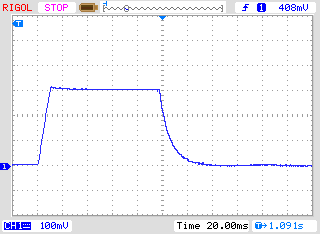
\includegraphics[width=9cm]{../PNG/charge_229uF.png}
    \caption{\(229\mu F\) Kondensator}
    \label{pic:c229}
  \end{subfigure}
  ~
  \begin{subfigure}[b]{9cm}
    \centering
    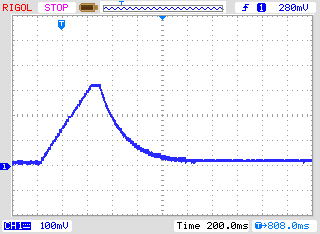
\includegraphics[width=9cm]{../PNG/charge_5mF.png}
    \caption{\(5mF\) Kondensator}
    \label{pic:c5mF}
  \end{subfigure}
  \caption{Laden und Entladen von gro"sen Kondensatoren f\"ur die Messung}
\end{figure}

\begin{figure}[H]
  \centering
    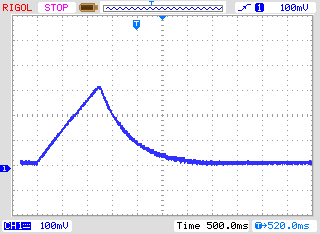
\includegraphics[]{../PNG/charge_15mF.png}
  \caption{Laden und Entladen eines \(15mF\) Kondensators f\"ur die Messung}
  \label{pic:c15mF}
\end{figure}

\subsection{Messen von kleinen Kapazit\"aten}
Wenn der erste 10 ms Ladepuls den Kondensator zu hoch aufgeladen hat, wird eine andere Me"stechnik benutzt.
Der ATmega Prozessor hat einen eingebauten 16-Bit Z\"ahler, der bei voller Taktfrequenz (1MHz oder 8MHz) arbeiten kann.
Diese Z\"ahler hat auch die F\"ahigkeit aufgrund eines externen Ereignisses den Z\"ahlerstand zu sichern.
Dieses Ereignis kann auch das Ausgangs-Signal des Komparators sein.
Der Komparator kann mit jeden ADC Eingangspin und der Spannungsreferenz (Band Gap Reference) arbeiten.
Schaltbild~\ref{fig:comparat} zeigt ein vereinfachtes Diagram der Me"ssituation.
So entlade ich den Kondensator, bereite den Komparator f\"ur den richtigen Pin Eingang vor, starte den Z\"ahler bei 0 und
starte sofort das Laden des Kondensators.
Dabei ist eine Seite des Kondensators mit GND die andere Seite \"uber den \(470k\Omega\) Widerstand mit VCC verbunden.
Nun pr\"ufe ich in einer Programm-Schleife, ob der Z\"ahler ein \"Uberlauf-Ereignis (overflow) oder ein
 externes Ereignis (input capture) meldet.
Die \"Uberlauf-Ereignisse z\"ahle ich bis ich ein externes Ereignis feststelle.
In diesem Fall halte ich den Z\"ahler an und pr\"ufe, ob ich noch einen zus\"atzlichen \"Uberlauf z\"ahlen mu"s, 
weil der Z\"ahler nicht mit dem externen Ereignis (input capture) angehalten werden kann.


Der Z\"ahlerstand des externen Ereignisses bildet zusammen mit dem \"Uberlaufz\"ahler die Gesamtzeit,
von der ich eine experimentell herausgefundene Konstante abziehe, um den Me"swerte-Offset zu beseitigen.
Ich wei"s nicht, ob diese Konstante f\"ur andere Leiterplatten angepasst werden mu"s.
Die aktuelle Software kann eine Tabelle mit der theoretischen Abh\"angigkeit der Ladezeit in Bezug auf die Komparator-Spannung ber\"ucksichtigen.
Die Tabelle hat einen Abstand von 50mV Schritten und wird interpoliert entsprechend der aktuellen Referenz-Spannung.
Diese Tabelle wird nur mit der Makefile Option WITH\_AUTO\_REF aktiviert.
Ich habe bemerkt, da"s die Referenz-Spannung immer etwas zu klein gemessen wird,
 deshalb kann man einen Zusatz mit der Makefile Option REF\_KORR angeben.
Die gemessene Referenz-Spannung wird dann mit dem angegebenen Korrekturwert (mV) korrigiert (addiert).
Wenn die Option WITH\_AUTO\_REF nicht benutzt wird, werden die Referenz-Spannungen entsprechend den Angaben in den
Datenbl\"attern ~\cite{ATmega8}~\cite{ATmega168} der ATmega8, ATmega88, ATmega168 und ATmega328 Prozessoren ber\"ucksichtigt.
Eine Beispielmessung von diesem Typ ist in Abbildung~\ref{pic:c22uF} dargestellt.
Die Me"szeit ist ungef\"ahr 2,6s weil der \(470k\Omega\) Widerstand f\"ur das Laden benutzt wird,
aber das Entladen geht in diesem Fall viel schneller als das Laden.

\begin{figure}[H]
\centering

\includegraphics[]{../FIG/Comparat.eps}
\caption{Messung kleiner Kapazit\"atswerte mit dem Komparator}
\label{fig:comparat}
\end{figure}

\begin{figure}[H]
  \centering
    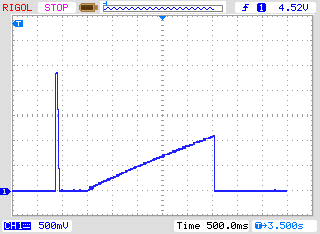
\includegraphics[]{../PNG/charge_22uF.png}
  \caption{Laden und Entladen eines \(22\mu F\) Kondensators f\"ur die Messung}
  \label{pic:c22uF}
\end{figure}


Im Prinzip kann diese Technik auch mit dem \(680\Omega\) Widerstand benutzt werden,
aber weil w\"ahrend dem Komparatorbetrieb der ADC nicht benutzt werden kann, habe ich keine
M\"oglichkeit die Ladespannung zu beobachten bis der Komparator angehalten wird.
Wenn eine unentdeckte Diode mit dem Kondensator parallelgeschaltet ist, kann der Ladestrom
von der Diode aufgenommen werden (Schwellspannung) und die Referenz-Spannung w\"urde nie erreicht.
Die Methode, die in der aktuellen Software f\"ur gro"se Kondensatoren in Kapitel~\ref{sec:bigcap}
verwendet wird, vermeidet diesen Konzeptfehler.

\subsection{Ergebnisse der Kondensator-Messung}
Die Ergebnisse meiner Messungen werden in Abbildung~\ref{fig:mega8cap} f\"ur den ATmega8 Prozessor ohne und mit
der AUTOSCALE\_ADC Option dargestellt. Zus\"atzlich sind einige Werte der Original-Software mit einem Korrekturfaktor
von 0,88~(-12\%) dargestellt.
Die Ergebnisse der Messung der gleichen Kondensatoren mit einem ATmega168 werden in Abbildung~\ref{fig:mega168cap} gezeigt.
Die Referenz f\"ur die Fehlerberechnung sind die Me"swerte eines PeakTech 2170 RCL-Me"sger\"ates, 
 nicht die aufgedruckten Werte der Bauteile.
Die gr\"o"seren relativen Me"sfehler bei gro"sen Kondensatoren liegen wahrscheinlich an der unterschiedlichen G\"ute 
der Elektrolytkondensatoren. Die G\"ute wird derzeit nicht ermittelt.

\begin{figure}[H]
\centering
% GNUPLOT: LaTeX picture with Postscript
\begingroup
  \makeatletter
  \providecommand\color[2][]{%
    \GenericError{(gnuplot) \space\space\space\@spaces}{%
      Package color not loaded in conjunction with
      terminal option `colourtext'%
    }{See the gnuplot documentation for explanation.%
    }{Either use 'blacktext' in gnuplot or load the package
      color.sty in LaTeX.}%
    \renewcommand\color[2][]{}%
  }%
  \providecommand\includegraphics[2][]{%
    \GenericError{(gnuplot) \space\space\space\@spaces}{%
      Package graphicx or graphics not loaded%
    }{See the gnuplot documentation for explanation.%
    }{The gnuplot epslatex terminal needs graphicx.sty or graphics.sty.}%
    \renewcommand\includegraphics[2][]{}%
  }%
  \providecommand\rotatebox[2]{#2}%
  \@ifundefined{ifGPcolor}{%
    \newif\ifGPcolor
    \GPcolortrue
  }{}%
  \@ifundefined{ifGPblacktext}{%
    \newif\ifGPblacktext
    \GPblacktexttrue
  }{}%
  % define a \g@addto@macro without @ in the name:
  \let\gplgaddtomacro\g@addto@macro
  % define empty templates for all commands taking text:
  \gdef\gplbacktext{}%
  \gdef\gplfronttext{}%
  \makeatother
  \ifGPblacktext
    % no textcolor at all
    \def\colorrgb#1{}%
    \def\colorgray#1{}%
  \else
    % gray or color?
    \ifGPcolor
      \def\colorrgb#1{\color[rgb]{#1}}%
      \def\colorgray#1{\color[gray]{#1}}%
      \expandafter\def\csname LTw\endcsname{\color{white}}%
      \expandafter\def\csname LTb\endcsname{\color{black}}%
      \expandafter\def\csname LTa\endcsname{\color{black}}%
      \expandafter\def\csname LT0\endcsname{\color[rgb]{1,0,0}}%
      \expandafter\def\csname LT1\endcsname{\color[rgb]{0,1,0}}%
      \expandafter\def\csname LT2\endcsname{\color[rgb]{0,0,1}}%
      \expandafter\def\csname LT3\endcsname{\color[rgb]{1,0,1}}%
      \expandafter\def\csname LT4\endcsname{\color[rgb]{0,1,1}}%
      \expandafter\def\csname LT5\endcsname{\color[rgb]{1,1,0}}%
      \expandafter\def\csname LT6\endcsname{\color[rgb]{0,0,0}}%
      \expandafter\def\csname LT7\endcsname{\color[rgb]{1,0.3,0}}%
      \expandafter\def\csname LT8\endcsname{\color[rgb]{0.5,0.5,0.5}}%
    \else
      % gray
      \def\colorrgb#1{\color{black}}%
      \def\colorgray#1{\color[gray]{#1}}%
      \expandafter\def\csname LTw\endcsname{\color{white}}%
      \expandafter\def\csname LTb\endcsname{\color{black}}%
      \expandafter\def\csname LTa\endcsname{\color{black}}%
      \expandafter\def\csname LT0\endcsname{\color{black}}%
      \expandafter\def\csname LT1\endcsname{\color{black}}%
      \expandafter\def\csname LT2\endcsname{\color{black}}%
      \expandafter\def\csname LT3\endcsname{\color{black}}%
      \expandafter\def\csname LT4\endcsname{\color{black}}%
      \expandafter\def\csname LT5\endcsname{\color{black}}%
      \expandafter\def\csname LT6\endcsname{\color{black}}%
      \expandafter\def\csname LT7\endcsname{\color{black}}%
      \expandafter\def\csname LT8\endcsname{\color{black}}%
    \fi
  \fi
  \setlength{\unitlength}{0.0500bp}%
  \begin{picture}(7200.00,5040.00)%
    \gplgaddtomacro\gplbacktext{%
      \csname LTb\endcsname%
      \put(814,704){\makebox(0,0)[r]{\strut{}-10}}%
      \csname LTb\endcsname%
      \put(814,1213){\makebox(0,0)[r]{\strut{}-5}}%
      \csname LTb\endcsname%
      \put(814,1722){\makebox(0,0)[r]{\strut{} 0}}%
      \csname LTb\endcsname%
      \put(814,2231){\makebox(0,0)[r]{\strut{} 5}}%
      \csname LTb\endcsname%
      \put(814,2740){\makebox(0,0)[r]{\strut{} 10}}%
      \csname LTb\endcsname%
      \put(814,3248){\makebox(0,0)[r]{\strut{} 15}}%
      \csname LTb\endcsname%
      \put(814,3757){\makebox(0,0)[r]{\strut{} 20}}%
      \csname LTb\endcsname%
      \put(814,4266){\makebox(0,0)[r]{\strut{} 25}}%
      \csname LTb\endcsname%
      \put(814,4775){\makebox(0,0)[r]{\strut{} 30}}%
      \csname LTb\endcsname%
      \put(946,484){\makebox(0,0){\strut{}10p}}%
      \csname LTb\endcsname%
      \put(1532,484){\makebox(0,0){\strut{}100p}}%
      \csname LTb\endcsname%
      \put(2117,484){\makebox(0,0){\strut{}1n}}%
      \csname LTb\endcsname%
      \put(2703,484){\makebox(0,0){\strut{}10n}}%
      \csname LTb\endcsname%
      \put(3289,484){\makebox(0,0){\strut{}100n}}%
      \csname LTb\endcsname%
      \put(3875,484){\makebox(0,0){\strut{}1u}}%
      \csname LTb\endcsname%
      \put(4460,484){\makebox(0,0){\strut{}10u}}%
      \csname LTb\endcsname%
      \put(5046,484){\makebox(0,0){\strut{}100u}}%
      \csname LTb\endcsname%
      \put(5632,484){\makebox(0,0){\strut{}1m}}%
      \csname LTb\endcsname%
      \put(6217,484){\makebox(0,0){\strut{}10m}}%
      \csname LTb\endcsname%
      \put(6803,484){\makebox(0,0){\strut{}100m}}%
      \put(176,2739){\rotatebox{-270}{\makebox(0,0){\strut{}Error / Percent}}}%
      \put(3874,154){\makebox(0,0){\strut{}Capacity value / F}}%
      \put(3874,4665){\makebox(0,0){\strut{}}}%
    }%
    \gplgaddtomacro\gplfronttext{%
      \csname LTb\endcsname%
      \put(2002,4602){\makebox(0,0)[r]{\strut{}Mega8}}%
      \csname LTb\endcsname%
      \put(2002,4382){\makebox(0,0)[r]{\strut{}Mega8as}}%
      \csname LTb\endcsname%
      \put(2002,4162){\makebox(0,0)[r]{\strut{}orig}}%
    }%
    \gplbacktext
    \put(0,0){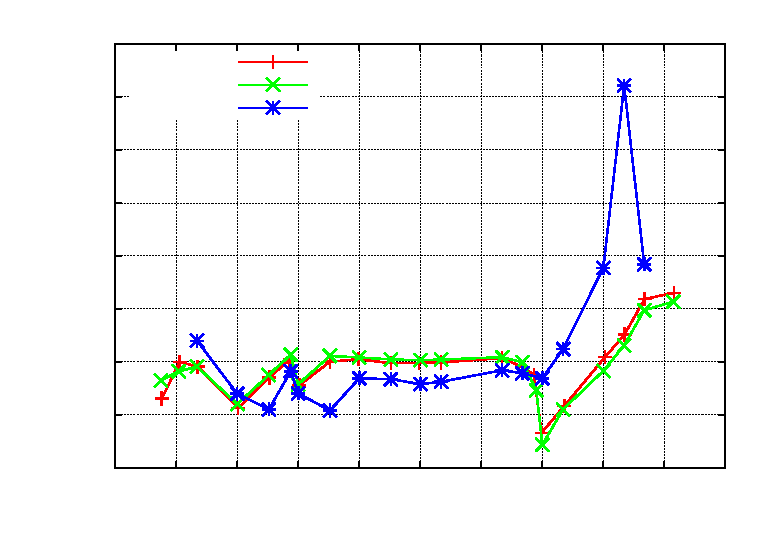
\includegraphics{../GNU/Mega8cap}}%
    \gplfronttext
  \end{picture}%
\endgroup

\caption{Prozentualer Fehler der Kondensator-Messungen mit dem ATmega8}
\label{fig:mega8cap}
\end{figure}

\begin{figure}[H]
\centering
% GNUPLOT: LaTeX picture with Postscript
\begingroup
  \makeatletter
  \providecommand\color[2][]{%
    \GenericError{(gnuplot) \space\space\space\@spaces}{%
      Package color not loaded in conjunction with
      terminal option `colourtext'%
    }{See the gnuplot documentation for explanation.%
    }{Either use 'blacktext' in gnuplot or load the package
      color.sty in LaTeX.}%
    \renewcommand\color[2][]{}%
  }%
  \providecommand\includegraphics[2][]{%
    \GenericError{(gnuplot) \space\space\space\@spaces}{%
      Package graphicx or graphics not loaded%
    }{See the gnuplot documentation for explanation.%
    }{The gnuplot epslatex terminal needs graphicx.sty or graphics.sty.}%
    \renewcommand\includegraphics[2][]{}%
  }%
  \providecommand\rotatebox[2]{#2}%
  \@ifundefined{ifGPcolor}{%
    \newif\ifGPcolor
    \GPcolortrue
  }{}%
  \@ifundefined{ifGPblacktext}{%
    \newif\ifGPblacktext
    \GPblacktexttrue
  }{}%
  % define a \g@addto@macro without @ in the name:
  \let\gplgaddtomacro\g@addto@macro
  % define empty templates for all commands taking text:
  \gdef\gplbacktext{}%
  \gdef\gplfronttext{}%
  \makeatother
  \ifGPblacktext
    % no textcolor at all
    \def\colorrgb#1{}%
    \def\colorgray#1{}%
  \else
    % gray or color?
    \ifGPcolor
      \def\colorrgb#1{\color[rgb]{#1}}%
      \def\colorgray#1{\color[gray]{#1}}%
      \expandafter\def\csname LTw\endcsname{\color{white}}%
      \expandafter\def\csname LTb\endcsname{\color{black}}%
      \expandafter\def\csname LTa\endcsname{\color{black}}%
      \expandafter\def\csname LT0\endcsname{\color[rgb]{1,0,0}}%
      \expandafter\def\csname LT1\endcsname{\color[rgb]{0,1,0}}%
      \expandafter\def\csname LT2\endcsname{\color[rgb]{0,0,1}}%
      \expandafter\def\csname LT3\endcsname{\color[rgb]{1,0,1}}%
      \expandafter\def\csname LT4\endcsname{\color[rgb]{0,1,1}}%
      \expandafter\def\csname LT5\endcsname{\color[rgb]{1,1,0}}%
      \expandafter\def\csname LT6\endcsname{\color[rgb]{0,0,0}}%
      \expandafter\def\csname LT7\endcsname{\color[rgb]{1,0.3,0}}%
      \expandafter\def\csname LT8\endcsname{\color[rgb]{0.5,0.5,0.5}}%
    \else
      % gray
      \def\colorrgb#1{\color{black}}%
      \def\colorgray#1{\color[gray]{#1}}%
      \expandafter\def\csname LTw\endcsname{\color{white}}%
      \expandafter\def\csname LTb\endcsname{\color{black}}%
      \expandafter\def\csname LTa\endcsname{\color{black}}%
      \expandafter\def\csname LT0\endcsname{\color{black}}%
      \expandafter\def\csname LT1\endcsname{\color{black}}%
      \expandafter\def\csname LT2\endcsname{\color{black}}%
      \expandafter\def\csname LT3\endcsname{\color{black}}%
      \expandafter\def\csname LT4\endcsname{\color{black}}%
      \expandafter\def\csname LT5\endcsname{\color{black}}%
      \expandafter\def\csname LT6\endcsname{\color{black}}%
      \expandafter\def\csname LT7\endcsname{\color{black}}%
      \expandafter\def\csname LT8\endcsname{\color{black}}%
    \fi
  \fi
  \setlength{\unitlength}{0.0500bp}%
  \begin{picture}(7200.00,5040.00)%
    \gplgaddtomacro\gplbacktext{%
      \csname LTb\endcsname%
      \put(814,704){\makebox(0,0)[r]{\strut{}-2}}%
      \csname LTb\endcsname%
      \put(814,1383){\makebox(0,0)[r]{\strut{} 0}}%
      \csname LTb\endcsname%
      \put(814,2061){\makebox(0,0)[r]{\strut{} 2}}%
      \csname LTb\endcsname%
      \put(814,2740){\makebox(0,0)[r]{\strut{} 4}}%
      \csname LTb\endcsname%
      \put(814,3418){\makebox(0,0)[r]{\strut{} 6}}%
      \csname LTb\endcsname%
      \put(814,4097){\makebox(0,0)[r]{\strut{} 8}}%
      \csname LTb\endcsname%
      \put(814,4775){\makebox(0,0)[r]{\strut{} 10}}%
      \csname LTb\endcsname%
      \put(946,484){\makebox(0,0){\strut{}10p}}%
      \csname LTb\endcsname%
      \put(1532,484){\makebox(0,0){\strut{}100p}}%
      \csname LTb\endcsname%
      \put(2117,484){\makebox(0,0){\strut{}1n}}%
      \csname LTb\endcsname%
      \put(2703,484){\makebox(0,0){\strut{}10n}}%
      \csname LTb\endcsname%
      \put(3289,484){\makebox(0,0){\strut{}100n}}%
      \csname LTb\endcsname%
      \put(3875,484){\makebox(0,0){\strut{}1u}}%
      \csname LTb\endcsname%
      \put(4460,484){\makebox(0,0){\strut{}10u}}%
      \csname LTb\endcsname%
      \put(5046,484){\makebox(0,0){\strut{}100u}}%
      \csname LTb\endcsname%
      \put(5632,484){\makebox(0,0){\strut{}1m}}%
      \csname LTb\endcsname%
      \put(6217,484){\makebox(0,0){\strut{}10m}}%
      \csname LTb\endcsname%
      \put(6803,484){\makebox(0,0){\strut{}100m}}%
      \put(176,2739){\rotatebox{-270}{\makebox(0,0){\strut{}Error / Percent}}}%
      \put(3874,154){\makebox(0,0){\strut{}Capacity value / F}}%
      \put(3874,4665){\makebox(0,0){\strut{}}}%
    }%
    \gplgaddtomacro\gplfronttext{%
      \csname LTb\endcsname%
      \put(2398,4602){\makebox(0,0)[r]{\strut{}Mega168}}%
      \csname LTb\endcsname%
      \put(2398,4382){\makebox(0,0)[r]{\strut{}Mega168as8}}%
    }%
    \gplbacktext
    \put(0,0){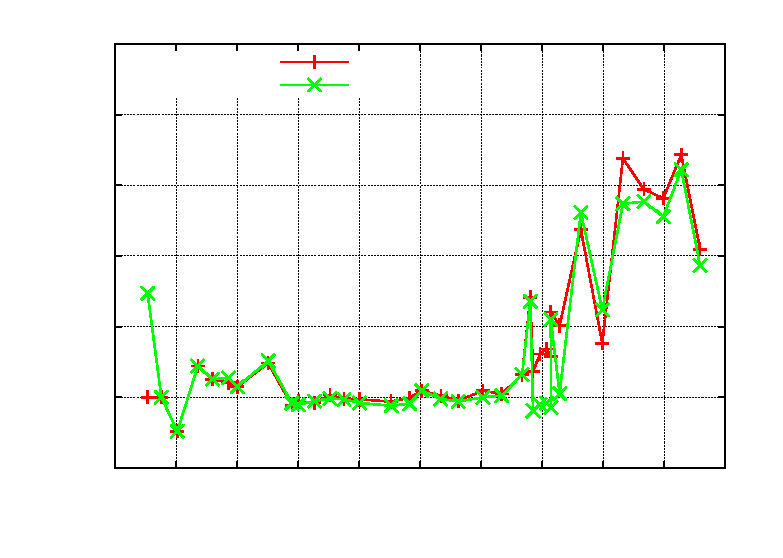
\includegraphics{../GNU/Mega168cap}}%
    \gplfronttext
  \end{picture}%
\endgroup

\caption{Prozentualer Fehler der Kondensator-Messungen mit dem ATmega168}
\label{fig:mega168cap}
\end{figure}

Die Abweichungen der Me"sergebnisse von drei verschiedenen ATmega168 Prozessoren und einem ATmega168A Prozessor werden in Abbildung~\ref{fig:mega168all} dargestellt.
Entsprechend werden die Me"sergebnisse von drei verschiedenen ATmega168A Prozessoren in Abbildungref{fig:mega168Aall} gezeigt.
Hierbei wurde nur der Nullwert der Kapazit\"atsmessung von 39pF ber\"ucksichtigt, alle anderen Korrekturm\"oglichkeiten wurden
nicht benutzt. Dieser Nullwert beinhaltet schon die 2-3pF, die durch die etwa 12~cm langen Anschlu"sleitungen mit den
Klemmem verursacht werden.
Auch das Board Layout hat Einflu"s auf diesen Nullwert. Diesen Nullwert habe ich mit der Board Version ,,DG2BRS V 5.2.1'' ermittelt.

\begin{figure}[H]
\centering
% GNUPLOT: LaTeX picture with Postscript
\begingroup
  \makeatletter
  \providecommand\color[2][]{%
    \GenericError{(gnuplot) \space\space\space\@spaces}{%
      Package color not loaded in conjunction with
      terminal option `colourtext'%
    }{See the gnuplot documentation for explanation.%
    }{Either use 'blacktext' in gnuplot or load the package
      color.sty in LaTeX.}%
    \renewcommand\color[2][]{}%
  }%
  \providecommand\includegraphics[2][]{%
    \GenericError{(gnuplot) \space\space\space\@spaces}{%
      Package graphicx or graphics not loaded%
    }{See the gnuplot documentation for explanation.%
    }{The gnuplot epslatex terminal needs graphicx.sty or graphics.sty.}%
    \renewcommand\includegraphics[2][]{}%
  }%
  \providecommand\rotatebox[2]{#2}%
  \@ifundefined{ifGPcolor}{%
    \newif\ifGPcolor
    \GPcolortrue
  }{}%
  \@ifundefined{ifGPblacktext}{%
    \newif\ifGPblacktext
    \GPblacktexttrue
  }{}%
  % define a \g@addto@macro without @ in the name:
  \let\gplgaddtomacro\g@addto@macro
  % define empty templates for all commands taking text:
  \gdef\gplbacktext{}%
  \gdef\gplfronttext{}%
  \makeatother
  \ifGPblacktext
    % no textcolor at all
    \def\colorrgb#1{}%
    \def\colorgray#1{}%
  \else
    % gray or color?
    \ifGPcolor
      \def\colorrgb#1{\color[rgb]{#1}}%
      \def\colorgray#1{\color[gray]{#1}}%
      \expandafter\def\csname LTw\endcsname{\color{white}}%
      \expandafter\def\csname LTb\endcsname{\color{black}}%
      \expandafter\def\csname LTa\endcsname{\color{black}}%
      \expandafter\def\csname LT0\endcsname{\color[rgb]{1,0,0}}%
      \expandafter\def\csname LT1\endcsname{\color[rgb]{0,1,0}}%
      \expandafter\def\csname LT2\endcsname{\color[rgb]{0,0,1}}%
      \expandafter\def\csname LT3\endcsname{\color[rgb]{1,0,1}}%
      \expandafter\def\csname LT4\endcsname{\color[rgb]{0,1,1}}%
      \expandafter\def\csname LT5\endcsname{\color[rgb]{1,1,0}}%
      \expandafter\def\csname LT6\endcsname{\color[rgb]{0,0,0}}%
      \expandafter\def\csname LT7\endcsname{\color[rgb]{1,0.3,0}}%
      \expandafter\def\csname LT8\endcsname{\color[rgb]{0.5,0.5,0.5}}%
    \else
      % gray
      \def\colorrgb#1{\color{black}}%
      \def\colorgray#1{\color[gray]{#1}}%
      \expandafter\def\csname LTw\endcsname{\color{white}}%
      \expandafter\def\csname LTb\endcsname{\color{black}}%
      \expandafter\def\csname LTa\endcsname{\color{black}}%
      \expandafter\def\csname LT0\endcsname{\color{black}}%
      \expandafter\def\csname LT1\endcsname{\color{black}}%
      \expandafter\def\csname LT2\endcsname{\color{black}}%
      \expandafter\def\csname LT3\endcsname{\color{black}}%
      \expandafter\def\csname LT4\endcsname{\color{black}}%
      \expandafter\def\csname LT5\endcsname{\color{black}}%
      \expandafter\def\csname LT6\endcsname{\color{black}}%
      \expandafter\def\csname LT7\endcsname{\color{black}}%
      \expandafter\def\csname LT8\endcsname{\color{black}}%
    \fi
  \fi
  \setlength{\unitlength}{0.0500bp}%
  \begin{picture}(7200.00,5040.00)%
    \gplgaddtomacro\gplbacktext{%
      \csname LTb\endcsname%
      \put(814,704){\makebox(0,0)[r]{\strut{}-4}}%
      \csname LTb\endcsname%
      \put(814,1111){\makebox(0,0)[r]{\strut{}-2}}%
      \csname LTb\endcsname%
      \put(814,1518){\makebox(0,0)[r]{\strut{} 0}}%
      \csname LTb\endcsname%
      \put(814,1925){\makebox(0,0)[r]{\strut{} 2}}%
      \csname LTb\endcsname%
      \put(814,2332){\makebox(0,0)[r]{\strut{} 4}}%
      \csname LTb\endcsname%
      \put(814,2740){\makebox(0,0)[r]{\strut{} 6}}%
      \csname LTb\endcsname%
      \put(814,3147){\makebox(0,0)[r]{\strut{} 8}}%
      \csname LTb\endcsname%
      \put(814,3554){\makebox(0,0)[r]{\strut{} 10}}%
      \csname LTb\endcsname%
      \put(814,3961){\makebox(0,0)[r]{\strut{} 12}}%
      \csname LTb\endcsname%
      \put(814,4368){\makebox(0,0)[r]{\strut{} 14}}%
      \csname LTb\endcsname%
      \put(814,4775){\makebox(0,0)[r]{\strut{} 16}}%
      \csname LTb\endcsname%
      \put(946,484){\makebox(0,0){\strut{}10p}}%
      \csname LTb\endcsname%
      \put(1597,484){\makebox(0,0){\strut{}100p}}%
      \csname LTb\endcsname%
      \put(2248,484){\makebox(0,0){\strut{}1n}}%
      \csname LTb\endcsname%
      \put(2898,484){\makebox(0,0){\strut{}10n}}%
      \csname LTb\endcsname%
      \put(3549,484){\makebox(0,0){\strut{}100n}}%
      \csname LTb\endcsname%
      \put(4200,484){\makebox(0,0){\strut{}1u}}%
      \csname LTb\endcsname%
      \put(4851,484){\makebox(0,0){\strut{}10u}}%
      \csname LTb\endcsname%
      \put(5501,484){\makebox(0,0){\strut{}100u}}%
      \csname LTb\endcsname%
      \put(6152,484){\makebox(0,0){\strut{}1m}}%
      \csname LTb\endcsname%
      \put(6803,484){\makebox(0,0){\strut{}10m}}%
      \put(176,2739){\rotatebox{-270}{\makebox(0,0){\strut{}Error / Percent}}}%
      \put(3874,154){\makebox(0,0){\strut{}Capacity value / F}}%
      \put(3874,4665){\makebox(0,0){\strut{}}}%
    }%
    \gplgaddtomacro\gplfronttext{%
      \csname LTb\endcsname%
      \put(5753,4602){\makebox(0,0)[r]{\strut{}168-1}}%
      \csname LTb\endcsname%
      \put(5753,4382){\makebox(0,0)[r]{\strut{}168-2}}%
      \csname LTb\endcsname%
      \put(5753,4162){\makebox(0,0)[r]{\strut{}168-3}}%
    }%
    \gplbacktext
    \put(0,0){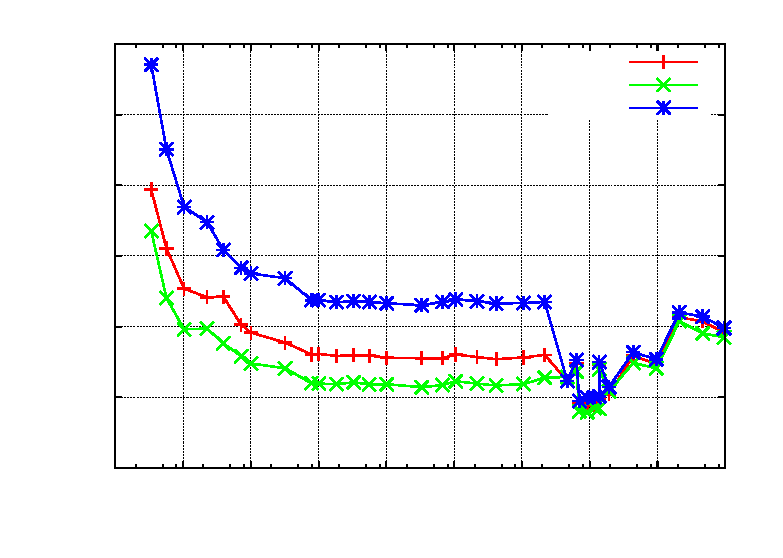
\includegraphics{../GNU/Mega168all}}%
    \gplfronttext
  \end{picture}%
\endgroup

\caption{Fehler der Kondensator-Messung von drei ATmega168 Prozessoren}
\label{fig:mega168all}
\end{figure}

\begin{figure}[H]
\centering
% GNUPLOT: LaTeX picture with Postscript
\begingroup
  \makeatletter
  \providecommand\color[2][]{%
    \GenericError{(gnuplot) \space\space\space\@spaces}{%
      Package color not loaded in conjunction with
      terminal option `colourtext'%
    }{See the gnuplot documentation for explanation.%
    }{Either use 'blacktext' in gnuplot or load the package
      color.sty in LaTeX.}%
    \renewcommand\color[2][]{}%
  }%
  \providecommand\includegraphics[2][]{%
    \GenericError{(gnuplot) \space\space\space\@spaces}{%
      Package graphicx or graphics not loaded%
    }{See the gnuplot documentation for explanation.%
    }{The gnuplot epslatex terminal needs graphicx.sty or graphics.sty.}%
    \renewcommand\includegraphics[2][]{}%
  }%
  \providecommand\rotatebox[2]{#2}%
  \@ifundefined{ifGPcolor}{%
    \newif\ifGPcolor
    \GPcolortrue
  }{}%
  \@ifundefined{ifGPblacktext}{%
    \newif\ifGPblacktext
    \GPblacktexttrue
  }{}%
  % define a \g@addto@macro without @ in the name:
  \let\gplgaddtomacro\g@addto@macro
  % define empty templates for all commands taking text:
  \gdef\gplbacktext{}%
  \gdef\gplfronttext{}%
  \makeatother
  \ifGPblacktext
    % no textcolor at all
    \def\colorrgb#1{}%
    \def\colorgray#1{}%
  \else
    % gray or color?
    \ifGPcolor
      \def\colorrgb#1{\color[rgb]{#1}}%
      \def\colorgray#1{\color[gray]{#1}}%
      \expandafter\def\csname LTw\endcsname{\color{white}}%
      \expandafter\def\csname LTb\endcsname{\color{black}}%
      \expandafter\def\csname LTa\endcsname{\color{black}}%
      \expandafter\def\csname LT0\endcsname{\color[rgb]{1,0,0}}%
      \expandafter\def\csname LT1\endcsname{\color[rgb]{0,1,0}}%
      \expandafter\def\csname LT2\endcsname{\color[rgb]{0,0,1}}%
      \expandafter\def\csname LT3\endcsname{\color[rgb]{1,0,1}}%
      \expandafter\def\csname LT4\endcsname{\color[rgb]{0,1,1}}%
      \expandafter\def\csname LT5\endcsname{\color[rgb]{1,1,0}}%
      \expandafter\def\csname LT6\endcsname{\color[rgb]{0,0,0}}%
      \expandafter\def\csname LT7\endcsname{\color[rgb]{1,0.3,0}}%
      \expandafter\def\csname LT8\endcsname{\color[rgb]{0.5,0.5,0.5}}%
    \else
      % gray
      \def\colorrgb#1{\color{black}}%
      \def\colorgray#1{\color[gray]{#1}}%
      \expandafter\def\csname LTw\endcsname{\color{white}}%
      \expandafter\def\csname LTb\endcsname{\color{black}}%
      \expandafter\def\csname LTa\endcsname{\color{black}}%
      \expandafter\def\csname LT0\endcsname{\color{black}}%
      \expandafter\def\csname LT1\endcsname{\color{black}}%
      \expandafter\def\csname LT2\endcsname{\color{black}}%
      \expandafter\def\csname LT3\endcsname{\color{black}}%
      \expandafter\def\csname LT4\endcsname{\color{black}}%
      \expandafter\def\csname LT5\endcsname{\color{black}}%
      \expandafter\def\csname LT6\endcsname{\color{black}}%
      \expandafter\def\csname LT7\endcsname{\color{black}}%
      \expandafter\def\csname LT8\endcsname{\color{black}}%
    \fi
  \fi
  \setlength{\unitlength}{0.0500bp}%
  \begin{picture}(7200.00,5040.00)%
    \gplgaddtomacro\gplbacktext{%
      \csname LTb\endcsname%
      \put(814,704){\makebox(0,0)[r]{\strut{}-10}}%
      \csname LTb\endcsname%
      \put(814,1156){\makebox(0,0)[r]{\strut{}-8}}%
      \csname LTb\endcsname%
      \put(814,1609){\makebox(0,0)[r]{\strut{}-6}}%
      \csname LTb\endcsname%
      \put(814,2061){\makebox(0,0)[r]{\strut{}-4}}%
      \csname LTb\endcsname%
      \put(814,2513){\makebox(0,0)[r]{\strut{}-2}}%
      \csname LTb\endcsname%
      \put(814,2966){\makebox(0,0)[r]{\strut{} 0}}%
      \csname LTb\endcsname%
      \put(814,3418){\makebox(0,0)[r]{\strut{} 2}}%
      \csname LTb\endcsname%
      \put(814,3870){\makebox(0,0)[r]{\strut{} 4}}%
      \csname LTb\endcsname%
      \put(814,4323){\makebox(0,0)[r]{\strut{} 6}}%
      \csname LTb\endcsname%
      \put(814,4775){\makebox(0,0)[r]{\strut{} 8}}%
      \csname LTb\endcsname%
      \put(946,484){\makebox(0,0){\strut{}10p}}%
      \csname LTb\endcsname%
      \put(1597,484){\makebox(0,0){\strut{}100p}}%
      \csname LTb\endcsname%
      \put(2248,484){\makebox(0,0){\strut{}1n}}%
      \csname LTb\endcsname%
      \put(2898,484){\makebox(0,0){\strut{}10n}}%
      \csname LTb\endcsname%
      \put(3549,484){\makebox(0,0){\strut{}100n}}%
      \csname LTb\endcsname%
      \put(4200,484){\makebox(0,0){\strut{}1u}}%
      \csname LTb\endcsname%
      \put(4851,484){\makebox(0,0){\strut{}10u}}%
      \csname LTb\endcsname%
      \put(5501,484){\makebox(0,0){\strut{}100u}}%
      \csname LTb\endcsname%
      \put(6152,484){\makebox(0,0){\strut{}1m}}%
      \csname LTb\endcsname%
      \put(6803,484){\makebox(0,0){\strut{}10m}}%
      \put(176,2739){\rotatebox{-270}{\makebox(0,0){\strut{}Error / Percent}}}%
      \put(3874,154){\makebox(0,0){\strut{}Capacity value / F}}%
      \put(3874,4665){\makebox(0,0){\strut{}}}%
    }%
    \gplgaddtomacro\gplfronttext{%
      \csname LTb\endcsname%
      \put(3282,3987){\makebox(0,0)[r]{\strut{}168A-4}}%
      \csname LTb\endcsname%
      \put(3282,3767){\makebox(0,0)[r]{\strut{}168A-5}}%
      \csname LTb\endcsname%
      \put(3282,3547){\makebox(0,0)[r]{\strut{}168A-6}}%
    }%
    \gplbacktext
    \put(0,0){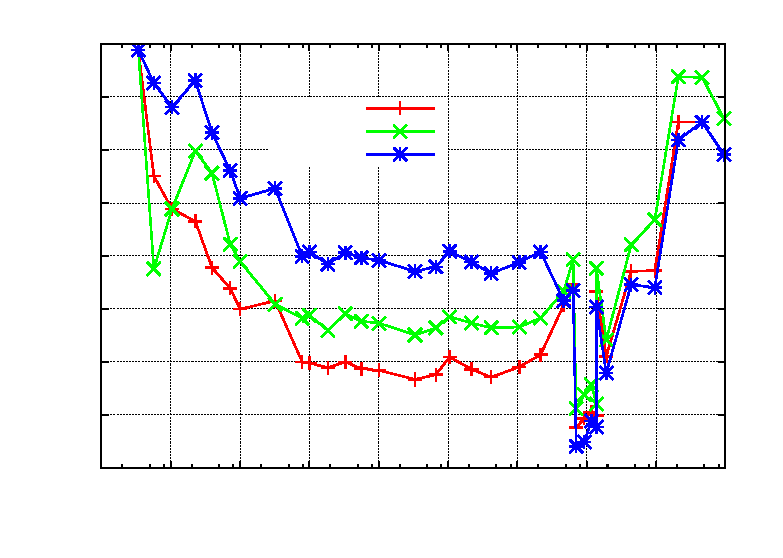
\includegraphics{../GNU/Mega168Aall}}%
    \gplfronttext
  \end{picture}%
\endgroup

\caption{Fehler der Kondensator-Messung von drei ATmega168A Prozessoren}
\label{fig:mega168Aall}
\end{figure}

Zum Erreichen der besten Me"sgenauigkeit mu"s die Software an die individuellen Eigenschaften des ATmega Exemplars
angepa"st werden. Dazu kann die Korrekturspannung REF\_C\_KORR f\"ur den Komparator angegeben werden, der f\"ur die Messung der kleinen 
Kapazit\"aten eingesetzt wird. Eine Korrekturspannung von 1mV f\"uhrt zu einer Verminderung der Kapazit\"atsanzeige von etwa 1~Promille.
F\"ur die gro"sen Kapazit\"aten kann der Promillewert C\_H\_KORR angegeben werden, um den die Messungen
zu gro"s sind. Da die gro"sen Kondensatoren meistens Elektrolytkondensatoren mit schechter G\"ute sind, ist die Bestimmung
des Kapazit\"atswertes und damit auch des Me"sfehlers hier besonders schwierig.
Besonders bei den ATmega168 Prozessoren habe ich bei kleinen Kapazit\"atswerten einen Me"sfehler beobachtet, 
der von der Anstiegsgeschwindigkeit der Spannung beim Ladevorgang abh\"angig ist.
Die Abbildung~\ref{fig:mega168optcap} zeigt die Me"sabweichung bei Kondensatormessung nur mit der Ber\"ucksichtigung des
Nullwertes (168-3-A), mit dem Korrekturfaktor f\"ur kleine Kondensatoren REF\_C\_KORR=66 sowie dem Korrekturfaktor f\"ur gro"se
Kondensatoren C\_H\_KORR=50 (168-3-B), sowie zus\"atzlich als Kurve 168-3-C  mit der Ber\"ucksichtigung einer Spannungsanstiegskomponente 
(COMP\_SLEW1=4000 und COMP\_SLEW2=220) und des Selbstentladeverhaltens der großen Kondensatoren.
Der Spannungsanstiegs-Korrekturfaktor berechnet sich nach \(\frac{COMP\_SLEW1}{cval+COMP\_SLEW2} - \frac{COMP\_SLEW1}{COMP\_SLEW2}\),
wobei cval der gemessene Kapazit\"atswert in pF ist.

\begin{figure}[H]
\centering
% GNUPLOT: LaTeX picture with Postscript
\begingroup
  \makeatletter
  \providecommand\color[2][]{%
    \GenericError{(gnuplot) \space\space\space\@spaces}{%
      Package color not loaded in conjunction with
      terminal option `colourtext'%
    }{See the gnuplot documentation for explanation.%
    }{Either use 'blacktext' in gnuplot or load the package
      color.sty in LaTeX.}%
    \renewcommand\color[2][]{}%
  }%
  \providecommand\includegraphics[2][]{%
    \GenericError{(gnuplot) \space\space\space\@spaces}{%
      Package graphicx or graphics not loaded%
    }{See the gnuplot documentation for explanation.%
    }{The gnuplot epslatex terminal needs graphicx.sty or graphics.sty.}%
    \renewcommand\includegraphics[2][]{}%
  }%
  \providecommand\rotatebox[2]{#2}%
  \@ifundefined{ifGPcolor}{%
    \newif\ifGPcolor
    \GPcolortrue
  }{}%
  \@ifundefined{ifGPblacktext}{%
    \newif\ifGPblacktext
    \GPblacktexttrue
  }{}%
  % define a \g@addto@macro without @ in the name:
  \let\gplgaddtomacro\g@addto@macro
  % define empty templates for all commands taking text:
  \gdef\gplbacktext{}%
  \gdef\gplfronttext{}%
  \makeatother
  \ifGPblacktext
    % no textcolor at all
    \def\colorrgb#1{}%
    \def\colorgray#1{}%
  \else
    % gray or color?
    \ifGPcolor
      \def\colorrgb#1{\color[rgb]{#1}}%
      \def\colorgray#1{\color[gray]{#1}}%
      \expandafter\def\csname LTw\endcsname{\color{white}}%
      \expandafter\def\csname LTb\endcsname{\color{black}}%
      \expandafter\def\csname LTa\endcsname{\color{black}}%
      \expandafter\def\csname LT0\endcsname{\color[rgb]{1,0,0}}%
      \expandafter\def\csname LT1\endcsname{\color[rgb]{0,1,0}}%
      \expandafter\def\csname LT2\endcsname{\color[rgb]{0,0,1}}%
      \expandafter\def\csname LT3\endcsname{\color[rgb]{1,0,1}}%
      \expandafter\def\csname LT4\endcsname{\color[rgb]{0,1,1}}%
      \expandafter\def\csname LT5\endcsname{\color[rgb]{1,1,0}}%
      \expandafter\def\csname LT6\endcsname{\color[rgb]{0,0,0}}%
      \expandafter\def\csname LT7\endcsname{\color[rgb]{1,0.3,0}}%
      \expandafter\def\csname LT8\endcsname{\color[rgb]{0.5,0.5,0.5}}%
    \else
      % gray
      \def\colorrgb#1{\color{black}}%
      \def\colorgray#1{\color[gray]{#1}}%
      \expandafter\def\csname LTw\endcsname{\color{white}}%
      \expandafter\def\csname LTb\endcsname{\color{black}}%
      \expandafter\def\csname LTa\endcsname{\color{black}}%
      \expandafter\def\csname LT0\endcsname{\color{black}}%
      \expandafter\def\csname LT1\endcsname{\color{black}}%
      \expandafter\def\csname LT2\endcsname{\color{black}}%
      \expandafter\def\csname LT3\endcsname{\color{black}}%
      \expandafter\def\csname LT4\endcsname{\color{black}}%
      \expandafter\def\csname LT5\endcsname{\color{black}}%
      \expandafter\def\csname LT6\endcsname{\color{black}}%
      \expandafter\def\csname LT7\endcsname{\color{black}}%
      \expandafter\def\csname LT8\endcsname{\color{black}}%
    \fi
  \fi
  \setlength{\unitlength}{0.0500bp}%
  \begin{picture}(7200.00,5040.00)%
    \gplgaddtomacro\gplbacktext{%
      \csname LTb\endcsname%
      \put(814,704){\makebox(0,0)[r]{\strut{}-5}}%
      \csname LTb\endcsname%
      \put(814,1286){\makebox(0,0)[r]{\strut{} 0}}%
      \csname LTb\endcsname%
      \put(814,1867){\makebox(0,0)[r]{\strut{} 5}}%
      \csname LTb\endcsname%
      \put(814,2449){\makebox(0,0)[r]{\strut{} 10}}%
      \csname LTb\endcsname%
      \put(814,3030){\makebox(0,0)[r]{\strut{} 15}}%
      \csname LTb\endcsname%
      \put(814,3612){\makebox(0,0)[r]{\strut{} 20}}%
      \csname LTb\endcsname%
      \put(814,4193){\makebox(0,0)[r]{\strut{} 25}}%
      \csname LTb\endcsname%
      \put(814,4775){\makebox(0,0)[r]{\strut{} 30}}%
      \csname LTb\endcsname%
      \put(946,484){\makebox(0,0){\strut{}10p}}%
      \csname LTb\endcsname%
      \put(1597,484){\makebox(0,0){\strut{}100p}}%
      \csname LTb\endcsname%
      \put(2248,484){\makebox(0,0){\strut{}1n}}%
      \csname LTb\endcsname%
      \put(2898,484){\makebox(0,0){\strut{}10n}}%
      \csname LTb\endcsname%
      \put(3549,484){\makebox(0,0){\strut{}100n}}%
      \csname LTb\endcsname%
      \put(4200,484){\makebox(0,0){\strut{}1u}}%
      \csname LTb\endcsname%
      \put(4851,484){\makebox(0,0){\strut{}10u}}%
      \csname LTb\endcsname%
      \put(5501,484){\makebox(0,0){\strut{}100u}}%
      \csname LTb\endcsname%
      \put(6152,484){\makebox(0,0){\strut{}1m}}%
      \csname LTb\endcsname%
      \put(6803,484){\makebox(0,0){\strut{}10m}}%
      \put(176,2739){\rotatebox{-270}{\makebox(0,0){\strut{}Error / Percent}}}%
      \put(3874,154){\makebox(0,0){\strut{}Capacity value / F}}%
      \put(3874,4665){\makebox(0,0){\strut{}}}%
    }%
    \gplgaddtomacro\gplfronttext{%
      \csname LTb\endcsname%
      \put(5753,4602){\makebox(0,0)[r]{\strut{}168-A}}%
      \csname LTb\endcsname%
      \put(5753,4382){\makebox(0,0)[r]{\strut{}168-B}}%
      \csname LTb\endcsname%
      \put(5753,4162){\makebox(0,0)[r]{\strut{}168-C}}%
    }%
    \gplbacktext
    \put(0,0){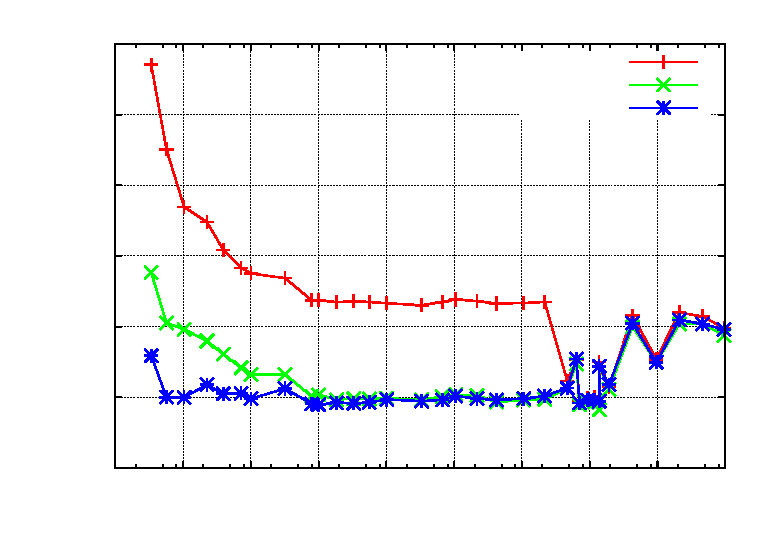
\includegraphics{../GNU/Mega168cap_opt}}%
    \gplfronttext
  \end{picture}%
\endgroup

\caption{Optimierung der Kondensator-Messung eines ATmega168}
\label{fig:mega168optcap}
\end{figure}
